	\subsection{Taxonomy of Virtualization Tools Taxonomy by \textit{Abdulhamid}}
	
	\begin{figure}[H]
		\centering
		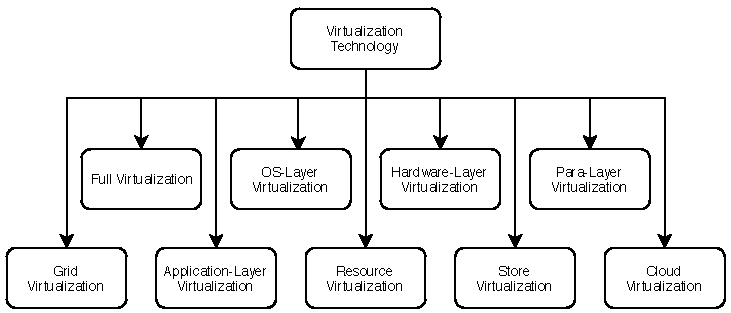
\includegraphics[width=8.5cm]{images/Abdulhamid2014.pdf}
		\vspace{-0.2cm}
		\caption{Taxonomy of virtualization tools by \textit{Shafi'i Muhammad Abdulhamid, Muhanmmad Shafie Abd Latiff and Mohammed Bakri Bashir} in 2014 \cite{Abdulhamid2014}.}
		\label{fig:TaxonomyByAbdulhamid}
	\end{figure}
	
	In the work of \textit{Abdulhamid} \cite{Abdulhamid2014} a taxonomy is presented whose purpose is to classify the hypervisors under the virtualization technology from the point of view of resource provisioning in cloud computing. 
	
	This initiative is supported by the boom in cloud computing, particularly infrastructure as a service (IaaS). 
	
	This purpose is based on the work of Sahoo, et al \cite{Sahoo2010}, which had the following seven categories: \textit{a) Full Virtualization}, \textit{b) OS-Layer Virtualization}, \textit{c) Hardware-Layer Virtualization}, \textit{d) Para virtualization}, \textit{e) Application virtualization}, \textit{f) Resource virtualization}, \textit{g) Storage virtualization}. In addition, \textit{Abdulhamid's} work adds the followings tow categories: \textit{h) Grid virtualization} and \textit{i) Cloud virtualization}. See Figure \ref{fig:TaxonomyByAbdulhamid}.
	
	Some of the categories proposed here have already been described, so below is brief description of only some of the remaining. 
	
	\textbf{Resource virtualization}
	
	\textbf{Grid virtualization}
	
	\textbf{Cloud virtualization}
	
	Although
	
	
